\chapter{Umsetzung}
\label{ch:S5_Umsetzung}

\section{Erläuterung des Softwaretechnischen Entwurfs}
\label{ch5:s:Entwurf}

Für die Softwaretechnische Umsetzung wurden zunächst die Anforderungen an das Geogameframework in Kapitel \ref{ch4:s:Lösungen} und die gewählte Lösung aus Kapitel \ref{ch4:s:choosen_solution} im Detail evaluiert. Für die Umsetzung des Entwurfs wurde zunächst ein Entwurfs des Prozesses identifiziert, welcher die Geodaten aus OSM bis hin zur Darstellung im Beispiel Spiel darstellt. Eine Visualisierung ist in Abbildung \ref{img:ch5_img01_framework_progress} zu sehen.
\\\\

\begin{figure}[H]
\begin{center}
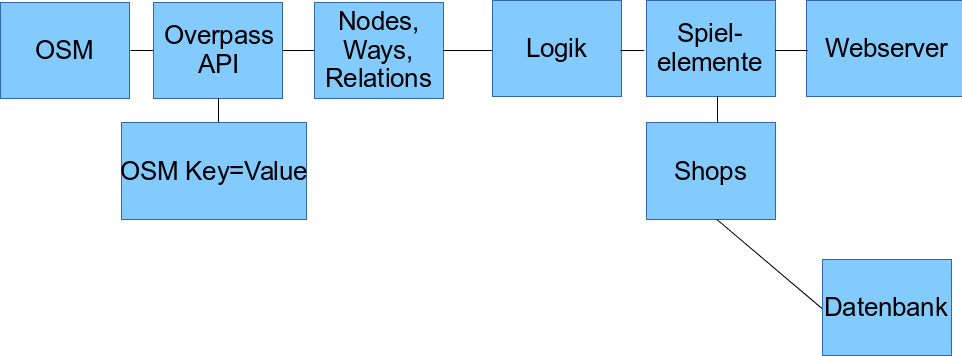
\includegraphics[width=140mm]{images/ch5_img01_framework_progress.png}
\caption{Prozess: Von OSM zum Spielelement}
\label{img:ch5_img01_framework_progress}
\end{center}
\end{figure}

\subsection*{OSM und Overpass API}

Zunächst steht zu Beginn des Prozesses als Datengrundlage OpenStreetMap.
Die Daten werden allerdings nicht direkt von OSM über die OSM API abgerufen, sondern über Overpass. Das liegt daran, dass die OSM API selbst nur sehr rudimentäre Abfragen erlaubt.
Stattdessen wird die Overpass API verwendet, da diese geografische Abfragen erlaubt.\cite{Meyer.2013}
Diese Abfragen sind notwendig, für die Anforderung notwendig, da die Spielelemente basierend auf einem OSM Key-Value Paar ausgelesen werden sollen. Darüber hinaus wird die Transformation der Relations und Ways in Nodes einfacher ermöglicht.
Durch die Verwendung der Overpass QL-Abfrage Sprache (OQL) ist es möglich nicht nur die jeweiligen Relations, Ways und Nodes eines Tags zu erhalten, sondern auch zusätzlich alle rekursiv enthaltenen Elemente. Dadurch erhält man den kompletten Datensatz mit einer Abfrage. Dieser ist für die spätere Transformation nötig. Der Vorteil liegt darin, dass nicht mehrere Abfragen gestartet werden müssen und sich somit die Zeit bis alle Daten zur Verfügung stehen, erheblich reduziert. Die Overpass API selbst bietet diverse Ausgabe-Formate wie XML und JSON.\cite{Olbricht.2014} Für eine konkrete Umsetzung wurde sich bewusst für JSON entschieden. JSON bietet eine deutlich höhere Performance bei der Verarbeitung von JSON Dokumenten im Vergleich zu XML Dokumenten.\cite{Nurseitov.2009} Darüber hinaus ist das Zielformat GeoJSON und es entfällt eine zusätzliche Transformation.
Der Aufruf der OverpassAPI erfolgt mittels einfacher REST-Abfrage:
\\\\
\url{http://overpass-api.de/api/interpreter?data=OQL_BEFEHL}
\\\\
Über den Parameter \glqq data\grqq{} wird der jeweilige OQL Befehl abgesetzt.
Für die Weiterverarbeitung der Daten wird im Anschluss das JSON Ergebnis vom Framework geparst und weiterverarbeitet.

\subsection*{Transformations Logik}

Die Transformation der Relations und Ways wird wie in Kapitel \ref{ch4:s:choosen_solution} umgesetzt. Eine Visualisierung ist in Abbildung \ref{img:ch5_img02_transform} zu sehen.

\begin{figure}[H]
\begin{center}
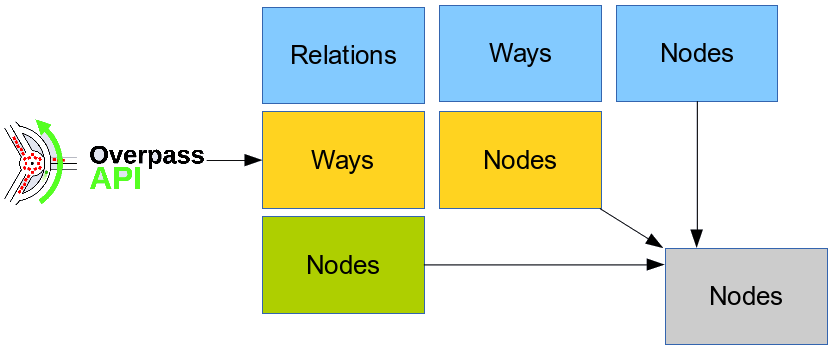
\includegraphics[width=140mm]{images/ch5_img02_transform.png}
\caption{Transformationsprozess: Relations, Ways, Nodes}
\label{img:ch5_img02_transform}
\end{center}
\end{figure}

Auf der linken Seite sind vertikal die Ausgangstypen angeordnet. Hierbei handelt es sich um die bereits angesprochenen Elemente Relations, Ways und Nodes. Im ersten Schritt werden die Daten der Overpass API aufbereitet. Danach werden alle Relations behandelt. Die Ways und Nodes, werden anschließend bearbeitet. Hiermit sollen zunächst alle Ways und Nodes identifiziert werden, welche direkt einer Relation angehören und keine separaten Spielelemente darstellen. Die Vorgehensweise ist damit begründet, dass die Anzahl der Anfragen für ein Spielfeld auf eine einzige reduziert wird. Somit enthält die Antwort alle Ways und Nodes. Die Nodes einer Relation, als auch die eines Ways, welche selbst nicht eigenständig sind werden zuerst ignoriert. Daher müssen die Elemente nacheinander, wie in Abbildung \ref{img:ch5_img02_transform} zu sehen, abgearbeitet werden.
\\\\
Zunächst werden alle Relationen bearbeitet. Für jede Relation werden nun die beinhalteten Ways und Nodes identifiziert. Relations selbst werden nicht rekursiv aufgelöst, da es nicht das Ziel ist möglichst wenige Spielelemente zu haben, sondern die Relationen zu transformieren. Sollten Relations mehreren Unterrelations haben, so sollen diese als Eigenständige Elemente betrachtet werden. Sofern sich dieser Ansatz  als nachteilig in der Evaluation herausstellt, muss er modifiziert werden.
Für die jeweilige Iteration eines Relation Elements werden alle beteiligten Ways und Nodes zu einer Liste von Nodes zusammengefasst. Diese Liste wird wiederum durch das in Kapitel \ref{ch4:s:choosen_solution} beschriebene Verfahren auf ein virtuelles Node reduziert. Hierzu wird für die Bounding Box der Mittelpunkt berechnet, welcher die Relation repräsentiert. Dieses virtuelle Node hat eine Koordinate, sowie eine ID welche es eindeutig identifizieren lässt. Hierzu wird die Relations ID von OSM verwendet.

Im nächsten Schritt werden die Ways abgearbeitet. Ways, die bereits in einer Relation enthalten sind, werden ignoriert. Alle anderen Ways werden jeweils zu einer Liste von Nodes und anschließend zu einem virtuellen Node transformiert. Hierbei entsteht wieder eine Koordinate und als ID wird die OSM Way ID verwendet.

Die als Node vorliegenden Elemente können direkt übernommen werden. Sie werden in Spielelemente, hier durch das graue Nodes Element symbolisiert, transferiert. Hierzu wird die Koordinate, sowie die OSM ID der Nodes übernommen.

Eine Problematik stellt sich in der eindeutigen Identifizierung der virtuellen Nodes. Da diese von unterschiedlichen Elementen (Relatons, Ways, Nodes) abgeleitet wurden, muss sichergestellt werden, dass anhand der ID eine eindeutige OSM Zuordnung möglich ist.
Entweder es wird zusätzlich der abgeleitete Typ des Spielelements explizit gespeichert oder man transcodiert die Information mit in die ID.
Wenn man sich zunächst die OSM IDs für Nodes anschaut, stellt man fest, dass diese die 32 Bit signed Integer Grenze überschritten haben (Februar 2013). Im OSM Wiki wird daher empfohlen den Datentyp long zu verwenden, welcher in den Standard-Implementierungen ein 64 Bit Wert ist.\cite{OSM.2013b}
Eine Möglichkeit den Typ des Spielelements zu übertragen ist die Verwendung einer Bitmaske, welche den Typ in der ID codiert. Hierzu könnte man die den 2. und 3. Bit eines 6 4 Bit long Wertes verwenden. Der 1. Bit wird nicht verwendet um negative Zahlen weiterhin zu erlauben. Der 2. Bit würde als Identifikator für Relations dienen und der 3. für Ways als Ursprungselement. Ein Beispiel für den transformierten Way mit der OSM ID 1 ist in Abbildung \ref{img:ch5_img03_bitmask} zu sehen.

\begin{figure}[H]
\begin{center}
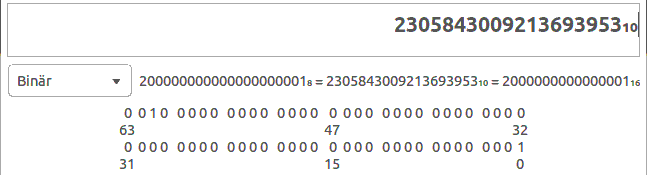
\includegraphics[width=120mm]{images/ch5_img03_bitmask.png}
\caption{OSM ID: Bitmaskenkodierung im 64 Bit long Wert}
\label{img:ch5_img03_bitmask}
\end{center}
\end{figure}


Wenn man die Reduzierung von 63 Bit (signed) auf 61bit(signed) mit der aktuellen Mapping Geschwindigkeit bei OSM vergleicht, so lässt sich feststellen, dass die Reduzierung um 2 Bit aus Paradigmensicht zwar unsauber erscheint, aber eine Überschreitung der ID \begin{math}2^{61}\end{math} in ferner Zukunft liegt. Zudem könnte im Bedarfsfall, wenn OSM auf 128 Bit IDs umsteigt, die Bitmaske angepasst werden.

\subsection*{Händler Integration}

Nachdem die virtuellen Nodes für die Spielelemente erstellt wurden, müssen die Elemente um die Händlern POIs ergänzt werden. In Kapitel \ref{ch4:s:choosen_solution} wurde erläutert, dass die Händler nicht als aktives Spielzielelement verwendet werden sollen, sondern als eine Integration der Händler und Dienstleister im Spiel als Repräsentation ihrer selbst.
Die Händler fungieren in diesem Zusammenhang als Anbieter für Items und andere Gegenstände. Für die spätere Darstellung auf der Karte müssen diese ebenfalls mit einer Koordinate versehen werden und separat behandelt werden. D.h. die Spielpunkte der Händler kommen stattdessen aus einer lokalen Datenbank. Dabei wird bewusst auf die Verwendung von OSM als Basis verzichtet. Zwar könnte man in einer erweiterten Version des Frameworks dem Nutzer unterstützen mit automatischen Vorschlägen basierend auf OSM, jedoch ist dies in der Grundfunktion nicht notwendig. Hier soll der Händler sich beliebig frei auf der Karte positionieren können und die Parameter seines virtuellen Geschäfts festlegen. Im Anschluss soll er die Items in seinem virtuellen Shop hinterlegen können. Da die Items eventuell vom Händler gegen einen Betrag vom Spielleiter erkauft werden, hat der Spielleiter ein  Interesse an der Verwendung der Items im Spiel. Allerdings muss auch sichergestellt werden, dass auf der anderen Seite das Spiel nicht in einen unausgeglichenen Zustand gerät. Wenn zu viele Spieler die Items eines Händlers bevorzugt werden, kann dies zu Frust bei den benachteiligten Spielern führen. Daher sollte es im Ermessen des Spielleiters liegen, dass dieser die Art und Verwendung der Items selbst definiert und Vorschläge für die Händler parat hat. Dass der Händler sich selbst mit Spielmechaniken und Balancing auseinander setzt, ist höchst unwahrscheinlich und würde nur zu mehr Koordinationsaufwand führen. Daher ist es am sinnvollsten dem Händler gewisse Items mit Standard-Eigenschaften anzubieten. Von diesen wiederum kann er einen Typ auswählen und eine Menge seinem virtuellen Shop zuordnen.
Für die Itemtypen kann der Spielleiter aller Voraussicht nach auf Erfahrungen seinerseits zurückgreifen. Darüber hinaus sollte das Framework ihm in einer erweiterten Ausbauphase auch Feedback über die Verwendung und Nutzung der Items aufzeigen. Aufgrund dieser Informationen können dann Rückschlüsse auf das Balancing gezogen werden.

\subsection*{Persistenz}

Ein wichtiger Aspekt des Frameworks stellt die Persistenz dar. Es müssen die Spielelemente, sowie der Spielzustand selbst gespeichert werden. Die Daten für die Spielelemente stammen aus OSM und von der lokalen Datenbank. Da die OSM-Daten transformiert werden, stellt sich die Frage ob dieser Prozess beschleunigt werden kann, wenn die Daten in der Datenbank lokal zwischengespeichert werden.
In Kapitel \ref{ch4:s:choosen_solution} ist bereits auf diesen Aspekt eingegangen worden. Die Problematik die sich durch eine Zwischenspeicherung stellt ist die Aktualisierung der Daten. Die lokalen Daten müssten mit einem Zeitstempel versehen und gehalten werden, bis diese \glqq verfallen\grqq. Darüber hinaus müssten diese nach dem Verfallszeitpunkt gelöscht oder aktualisiert werden. Ein Caching kann sinnvoll sein, sofern das Framework für ein Spiel mit einer kritischen Masse an Spielern verwendet wird. Allerdings ist eine Evaluation und Untersuchung des Frameworks auf Hochskalierbarkeit nicht Bestandteil der ersten Ausbaustufe. Ein weiterer Aspekt stellt die Datenmenge dar. Sofern im Framework alle abgefragten OSM-Daten in der Datenbank hinterlegt werden, ohne dass diese eine Zustandsveränderung erfahren haben, ist dies zwar modelltechnisch korrekt, allerdings aus Performance und Platzgründen nicht zu empfehlen.
Da das Framework dem Spielleiter so wenig Aufwand wie möglich machen soll, ist zu verhindern, dass dieser sich um die Datenbank und Speicherplatz Probleme kümmern muss. Ein gutes Beispiel hierfür stellt auch das OSM Projekt selbst dar. Die bekannte Kartendarstellung verwendet zur Anzeige die Tiles. Diese Tiles werden auf Basis der OSM-Daten gerendert. Ein erster Ansatz wäre das Rendern aller Tiles.
Allerdings dauert der Renderprozess mehrere Tage und Aktualisierungen auf der Karte würden immer nur mit mehreren Tagen Verzögerung angezeigt werden. Hinzu kommt die Tatsache, dass nur ein Bruchteil der Kartendaten auch tatsächlich angeschaut wird (<2\% \cite{Haklay.2008}). Daher werden die Karten-Bilddaten in Echtzeit gerendert und nach einer gewissen Zeit wieder verworfen.
Daher ist es auch beim Framework nicht sinnvoll alle Daten zu speichern, sondern nur die Spielelemente mit denen ein Spieler aktiv interagiert.
Die Daten der Händler werden separat gespeichert. Sie befinden sich ebenfalls in einer Datenbank, besitzen allerdings im Vergleich zu den Spielelementen eine Persistenz unabhängig von ihrer Interaktion mit den Spielern.


\subsection*{Schnittstellen}

Ein Framework benötigt passende Schnittstellen über die es Funktionen und Daten nach Außen hin zur Verfügung stellt. Zunächst muss geklärt werden, wie die Daten verwendet werden sollen. Für das Beispiel Spiel ist die Darstellung der Karte über eine Website vorgesehen. Unabhängig von der später verwendeten Technologie müssen in diesem Fall sowohl die Spielelemente, als auch die Händlerdaten vom Framework zur Verfügung gestellt werden.

Zur Verdeutlichung wird an dieser Stelle die Entscheidung für eine Technologie in Abbildung \ref{img:ch5_img04_interfaces} auf das nachfolgende Kapitel verlegt.

\begin{figure}[H]
\begin{center}
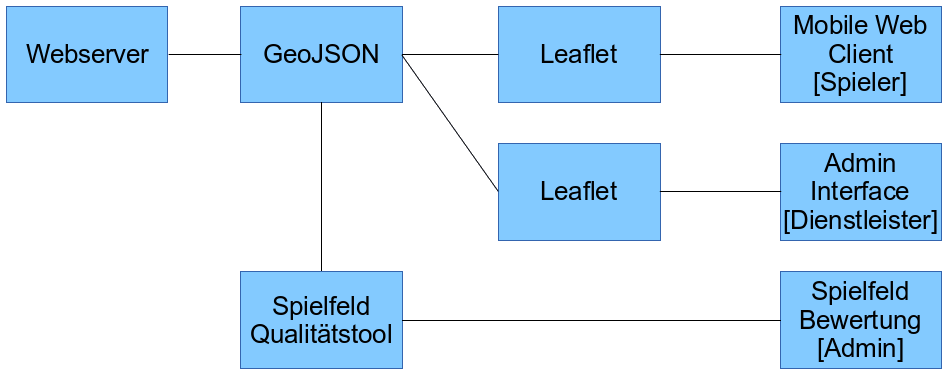
\includegraphics[width=140mm]{images/ch5_img04_interfaces.png}
\caption{Visualisierte Schnittstellen des Frameworks}
\label{img:ch5_img04_interfaces}
\end{center}
\end{figure}

Die Wahl des Formats für den Export der Spielelemente und Händlerdaten ist auf GeoJSON gefallen.
Dies ist mit den Daten von OSM und Overpass, welche als JSON im Framework ausgelesen werden begründet. Darüber hinaus verwendet eine Vielzahl der aktuellen Frameworks und Tools dieses Format. Während das offene Format WKT für die reine Repräsentation von Geodaten dient,\cite{Stolze.2003} bietet das GeoJSON Format zusätzlich die Möglichkeit Properties in einem Geo Objekt zu speichern.\cite{Butler.2008} Über diese kann wiederum das Framework Informationen wie z.\,B. die codierte OSM ID und Informationen zum Spielelement übertragen.
\\\\
Generell werden die Informationen des Frameworks für drei verschiedene Module benötigt.
Zunächst einmal gibt es den Spielclient bzw. dessen Oberfläche. Dieser benötigt die Daten für das Staging des Spiels selbst.
Über die Spieloberfläche interagiert der Spieler mit dem Spiel. Er sieht die aktuelle Karte, sowie die darauf platzierten Objekte. In diesem Fall sind dies die Spielelemente sowie die einzelnen Händler. Die Spielelemente selbst stellen im Beispiel Spiel die sogenannten Prestige Flaggen dar.

Ein weiteres Modul stellt die Administrationsoberfläche dar. Diese dient dem Spielleiter sowie dem jeweiligen Händler zur Konfiguration des Spiels. Im Detail kann der Spielleiter die Spielitems definieren, neue Händler anlegen und diese auf der Karte positionieren. Der Händler kann seine Metadaten pflegen und die Items, welche er in seinem virtuellen Laden anbieten möchte, selektieren. Bei Fehlern oder Aktualisierungen kann der jeweilige Administrator (Spielleiter oder Händler) diese problemlos anpassen. Für die Positionierung der virtuellen Läden auf der Karte wird ebenfalls analog zum Spielfeld eine GeoJSON Schnittstelle zum Einsatz kommen.

Das letzte Modul stellt die Evaluierung der Spielfelder dar. Hierbei wird die gleiche Schnittstelle verwendet, wie für die Aufbereitung des Spielfeldes. Das Tool bietet die Möglichkeit die importierten Spielfelder mit einem Algorithmus zu bewerten. Dieses Tool wird in Kapitel \ref{ch:CH6_qualtiy_of_gameboards} in vorgestellt. Über dieses wird das ideale Key-Value Paar für die OSM Tag Selektion eines Spielfeldes evaluiert. Dies soll dem Spielleiter die Möglichkeit einer objektiven Bewertung der Spielfelder ermöglichen.

\subsection*{Darstellung}

Da das Framework für ortsbezogene Spiele verwendet werden soll, ist es daher unerlässlich dem Spieler und den Administratoren eine Visualisierung zu bieten. Zunächst gibt es das Spielfeld. Das Spielfeld verwendet im Hintergrund Kartenmaterial von OSM, auf das die einzelnen Elemente platziert werden. Die Karte selbst wird initial auf die (GPS-)Korrdinaten der Spielerposition zentriert. Dadurch ist es dem Spieler möglich sich direkt von seiner Position aus zu orientieren. Die auf der Karte eingezeichneten Elemente, wie Flaggen und Händler, kann der Spieler problemlos identifizieren und zu Fuß aufsuchen. In Abbildung \ref{img:ch5_img05_dialog} ist ein Mockup der Kartenoberfläche zu sehen. Je nach Flaggenstatus werden die Flaggen unterschiedlich farbig dargestellt. Das Ziel ist es neutrale Flaggen grau, feindliche Rot und eigene grün darzustellen. Damit erhält der Spieler automatisch einen Überblick über die Situation und kann auch durch das Zoomen auf der Karte seine weiteren Spielzüge planen.
Neben den Spielelementen werden dem Spieler die aktuellen Punkte angezeigt. Diese werden im Beispiel Spiel durch das einfache Addieren der Prestige der Flaggen im Spielerbesitz berechnet. Des weiteren wird dem Spieler eine Auswahl für sein Inventar angezeigt werden.
Über dieses kann er sich nicht nur alle Items in seinem Besitz anzeigen lassen, sondern auch diese verwenden. In einem späteren Ausbau des Frameworks sollen darüber hinaus Items mit anderen Spielern getauscht werden können.
Sofern der Spieler mit einer Flagge interagiert, wird ihm die aktuelle Prestigezahl der Flagge angezeigt. Je nachdem ob ihm die Flagge bereits gehört oder diese einem fremden Spieler angehörig ist, kann der Spieler diese \glqq angreifen\grqq{}. Durch den Angriff werden die Aktionspunkte des Spielers auf die Flagge transferiert. Ist die Flagge im Besitzt eines anderen Spielers, so sieht der Spieler dies durch die aktuelle Farbgebung und kann durch den Einsatz seiner Aktionspunkte die Prestigezahl reduzieren, was direkt angezeigt wird. Für die Interaktion mit den Händlern steht dem Spieler ein Menü zur Verfügung. Dieses erscheint, sobald der Spieler auf einen Händler klickt. Danach öffnet sich ein Menü über das der Spieler eine Übersicht der verfügbaren Items und deren Spielpreise erhält. Sollte der Händler Items, wie in Kapitel \ref{ch4:s:choosen_solution} beschrieben Coupons anbieten, so kann der Spieler diese an gegebener Stelle eingeben.

\begin{figure}[H]
\begin{center}
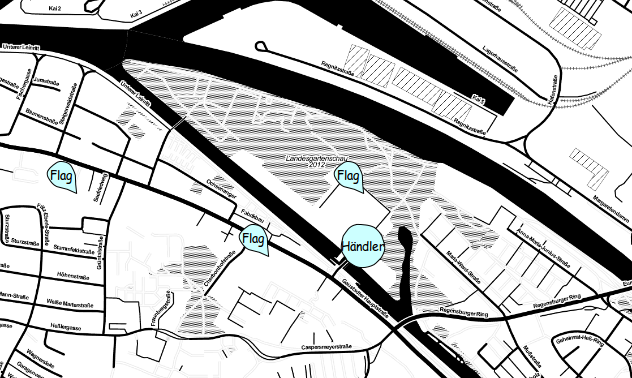
\includegraphics[width=140mm]{images/ch5_img05_dialog.png}
\caption{Spielfeld Mockup}
\label{img:ch5_img05_dialog}
\end{center}
\end{figure}

Der Administrationsbereich für den Spielleiter und den Händler arbeitet separat vom Spielfeld.
Je nachdem, ob Items oder Händler im System gepflegt werden sollen, wird dem Benutzer eine passende Liste präsentiert.
Beim Items Menü erhält der Benutzer eine Übersicht über alle Items die dem Spiel zur Verfügung stehen. Hierbei handelt es sich allerdings nicht um Itemtypen sondern direkt um die instantiierten Items selbst. Die Idee dahinter ist es, dem Spiel die Möglichkeit zu bieten auch einzigartige Items zu enthalten und sicherzustellen, dass ein Item jeweils auch immer als solches im System behandelt wird. Über die Liste gibt es die Option die bestehenden Items zu modifizieren oder zu entfernen. Neue Items können über eine Schaltfläche angelegt werden. Dabei wird dem Benutzer eine Oberfläche präsentiert und über Metadaten das Item genauer spezifiziert. Hier können der Name, Itemtyp und der dafür zu zahlende Preis gepflegt werden.
\\\\
Möchte der Benutzer dahingegen Händler pflegen, so erhält er zunächst analog zu den Items eine Übersicht der einzelnen Händler.
Diese kann er analog zu den Items modifizieren und löschen. Das Anlegen eines neuen Händlers ist genauso aufgebaut wie bei den Items. Der Unterschied liegt jedoch darin, dass es sich bei den Händlern nicht um einfache Formularfelder handelt, sondern auch zusätzlich eine Georepräsentation stattfinden muss. D.h. es muss die Positionierung des Händlers auf einer Karte erfolgen. Hierzu wird eine Art \glqq Picker\grqq{} verwendet. Auf einer OSM Karte soll der Benutzer die Position des Händlers definieren. Für eine Korrektur der Position reicht es aus, wenn der Benutzer einfach den Marker auf der Karte mit der Maus ergreift und per Drag and Drop auf seine neue Position bewegt.

%%\subsection*{Sonstige Funktionalitäten}


\subsection*{Technischer Entwurf}

Nachdem die Anforderungen beschrieben wurden, muss der softwaretechnische Entwurf konkretisiert werden.
Um die Software abzubilden zu können muss zunächst ein Modell entworfen werden, welches die Software abbildet. Die Prozesse des Frameworks wurden bereits in Abbildung \ref{img:ch5_img01_framework_progress} sowie \ref{img:ch5_img04_interfaces} visualisiert.

Zu Beginn einer Systementwicklung müssen die Usecases und die beteiligten Akteure identifiziert werden.
Hierfür wurde zu Beginn überlegt, welche Personen Zugang zum System haben sollen und welche Aufgaben diese am System erfüllen.
Dadurch wird sichergestellt, dass alle Aspekte behandelt werden, nicht nur die im initialen Lösungsansatz. Diese sind wichtig für den späteren Entwurf des Systems, sowie deren Umsetzung.
Die Usecases lassen sich als Diagramm wie in Abbildung \ref{img:ch5_img06_usecases} sichtbar definieren.



\begin{figure}[H]
\begin{center}
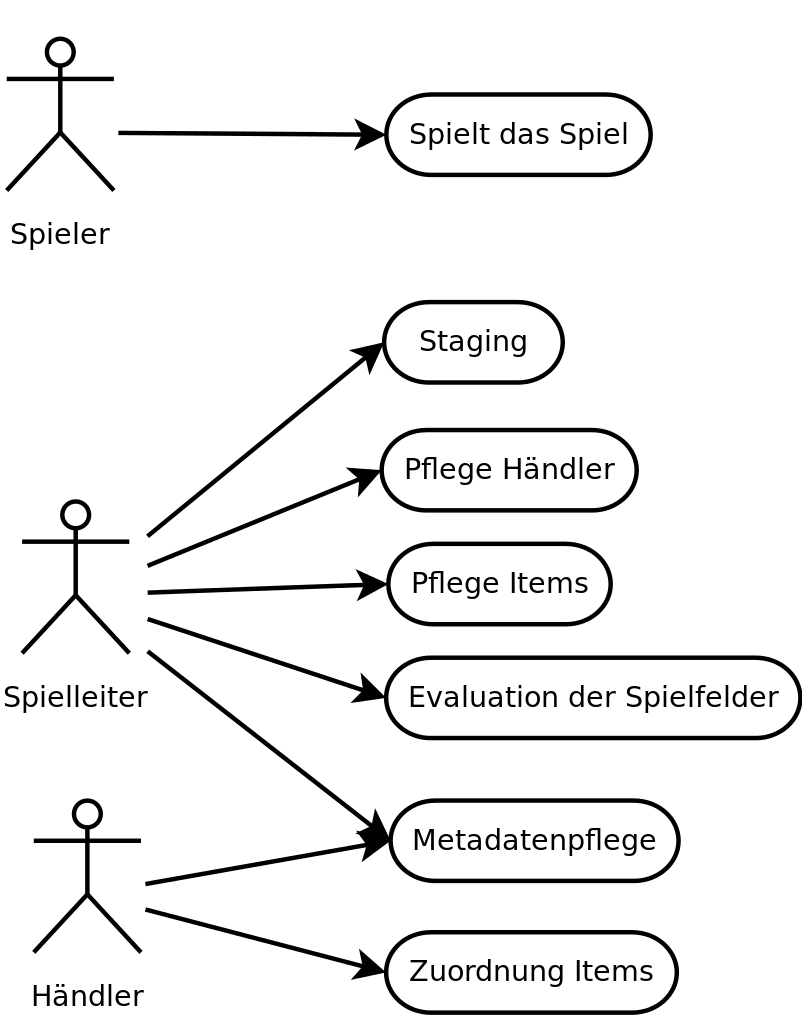
\includegraphics[width=100mm]{images/ch5_img06_usecases.png}
\caption{Usecase Diagramm}
\label{img:ch5_img06_usecases}
\end{center}
\end{figure}

Zunächst lässt sich feststellen, dass es drei Akteure gibt.
Diese decken sich soweit mit dem Lösungsansatz.
Der Spieler hat das Ziel das Spiel zu spielen. Der Spielleiter hingegen sieht es vor die Durchführung des Spiels mit dem Framework zu bewerkstelligen.
Hier muss er die Händler als auch Items pflegen. Darüber hinaus teilt er sich mit dem Händler die Metadatenpflege, da je nach Situation der Spielleiter mehr oder weniger in die individuelle Pflege der Händlerdaten eingebunden ist. Der Händler möchte zusätzlich seine Items, die er vom Spielleiter zugewiesen bekommen hat, auf seine virtuellen Läden verteilen. In der Grundfunktion des Framesworks sind nur diese Benutzer vorgesehen. In einer zweiten Ausbaustufe des Frameworks ist es sinnvoll explizite Nutzerrollen einzuführen um eine detailliertere Rechtezuweisung zu ermöglichen.
\\\\
Durch die Verwendung einer objektorientierten Programmiersprache ist es notwendig die dazugehörigen Klassen zu definieren.
Diese dienen dazu, Objekte abzuleiten und die jeweiligen Methoden von diesen zu nutzen.
Es muss sichergestellt werden, dass die Beziehungen zwischen den Klassen modular sind, damit ein einfacher Zugriff und eine Austauschbarkeit gegeben ist.
Um einen Einblick in die Struktur des Frameworks zu erhalten wird in diesem Abschnitt kurz auf die wichtigsten Aspekte eingegangen.


\begin{figure}[H]
\begin{center}
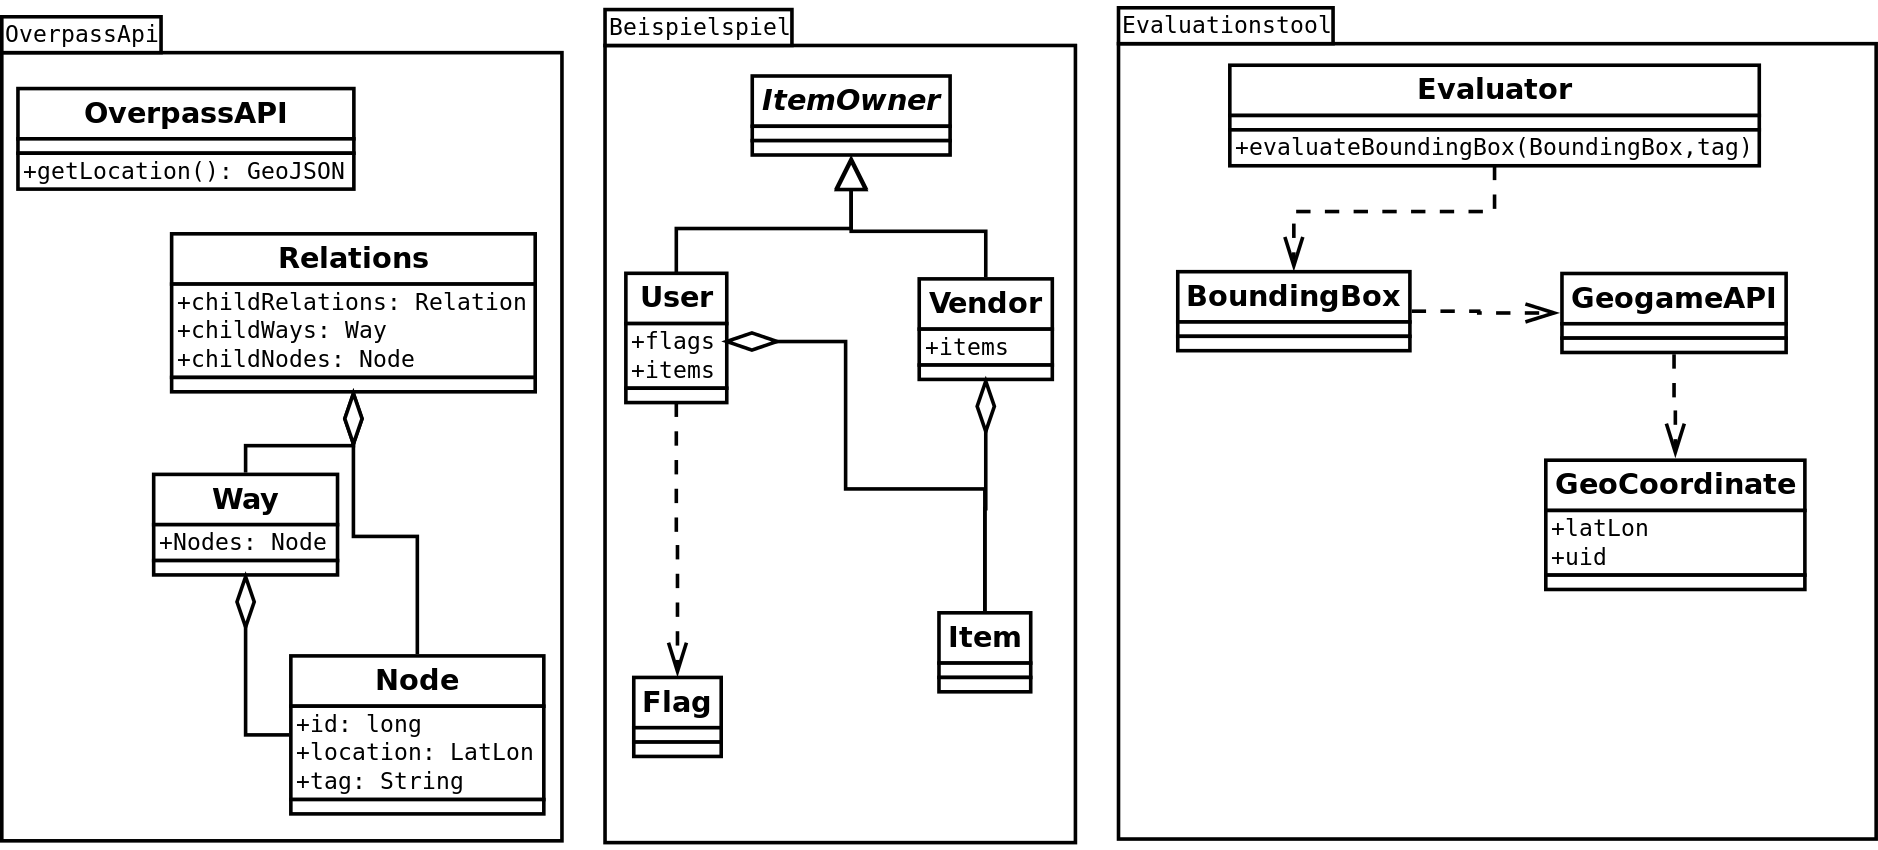
\includegraphics[width=150mm]{images/ch5_img07_classes.png}
\caption{Vereinfachtes Klassen Diagramm}
\label{img:ch5_img07_classes}
\end{center}
\end{figure}

In Abbildung \ref{img:ch5_img07_classes} ist ein vereinfachtes Klassendiagramm des Frameworks zu sehen. Das Framework als solches besteht aus drei Modulen. Zunächst gibt es den Bereich GameAPI. Es handelt sich nicht um die OverpassApi selbst, da Overpass selbst nur eine Webschnittstelle ist. Die beschriebene API ist die Implementierung der Schnittstelle im Framework selbst. Sie liefert das Ergebnis Transformation der Elemente Relations, Ways und Nodes aus dem Ergebins der Overpass-API. Diese werden wiederum durch den bereits beschriebenen Ansatz transformiert, in dem eine Umcodierung in virtuelle Nodes erfolgt. Im gleichen Zug wird überprüft, ob es persistierte Daten für die virtuellen Nodes in der lokalen Datenbank gibt. Sind passende Daten vorhanden, so werden die virtuellen Nodes um die jeweiligen Properties ergänzt und anschließend als JSON bzw. GeoJSON ausgegeben.
Im Anschluss werden diese über die Webschnittstelle des eigenen Frameworks ausgegeben.
Für die Händler gibt es eine separate Schnittstelle im Framework, welche analog zur Overpass Implementierung fungiert.
Die Daten sind nicht von Extern, sondern direkt in der fertigen Form aus der lokalen Datenbank.
Zudem ist auch keine Transformation notwendig, da die Elemente bereits als fertige Nodes vorliegen. Dies ist möglich, da jeder Händler nur als einziger Punkt im Spiel repräsentiert wird.
\\\\
Das nächste Modul ist das Beispiel Spiel. Das Beispiel Spiel selbst wurde einfach gehalten, da es zum einen als Proof of Conecept des Frameworks dienen soll und zum anderen der Fokus auf die Verteilung der Spielelemente auf dem Spielbrett untersucht werden soll.
Es gibt vier verschiedene Objekte. Spieler, Händler, Flaggen und Items.
Spieler und Händler stehen in einer polymorphen Verbindung zu Item. Beide Klassen leiten von einer abstrakten Klasse ItemOwner ab, welche Methoden vorhält die für die Interaktion als ItemOwner essentiell sind. Beispielsweise der Verkauf oder die Benutzung eines Items. Ein Item kann nur einem Spieler oder einem Händler angehören, niemals aber beiden gleichzeitig. Es gibt darüber hinaus die Möglichkeit, dass ein Item ohne ItemOwner existiert. Ein Beispiel könnte es sein, dass der Spielleiter für ein Event bestimmte Items auf der Karte ablegt oder zwei Spieler Items miteinander tauschen möchten.
\\\\
Das letzte Modul stellt das sogenannte Evalutationstool dar.
Mit diesem sollen die erzeugten Spielfelder analysiert und bewertet werden. Eine genauere Erläuterung der Funktionsweise ist in Kapitel \ref{ch:CH6_qualtiy_of_gameboards} zu finden.
Das Evaluationstool gereift zunächst auf die GeoJSON Schnittstelle des Frameworks zu. Dieses liefert bei einer Abfrage mittels Bounding Box und des OSM Tags, die Spielelemente zurück. Die Bounding Box wird auf Basis einer initialen Koordinate berechnet. Somit kann der Spielleiter einfach zwei Koordinaten definieren zu denen er gerne eine Auswertung interessanter Tags erhalten möchte. Das Evaluationstool startet im Anschluss den Vorgang und wandelt die Spielelemente in vereinfachte Objekte mit ID und Geo-Koordinaten um. Diese wiederum werden der jeweiligen Evaluationsmethode als Liste übergeben und deren Rückgabewert beschreibt die Kombination aus Bounding Box und OSM Tag.

\subsubsection*{Datenbank}

Aufgrund der vorherigen Analysen wird normalerweise ein Entity-Relationship-Modell (ERM) erstellt. Allerdings soll der Einsatz eines Webframeworks erfolgen, welches ein Objektrelationales Mapping unterstützt und somit die manuelle Erstellung der Datenbankstruktur nicht vorgesehen ist. Dies wird unter der Annahme gemacht, dass das Framework später im Produktiv-Betrieb für die Datenspeicherung optional auf eine NoSQL Lösung umgestellt werden kann. Diese bieten eine bessere Performance bei einfachen Abfragen.
Damit soll der, in der Literatur häufig kritisierte, Mismatch zwischen objektorientierter Programmierung und relationalen Datenbanken entgegnet werden.\cite{Cattell.1991}

Die geringe Verbreitung der objektorientierten Datenbanken liegt darin, dass nicht
versucht wurde die bestehenden Datenbanken zu ersetzten. Stattdessen sind die bereits existierenden Datenbanken in Unternehmen nicht in neue objektorientierte Datenbanken transferiert worden. Der Grund hierfür liegt in den historisch gewachsenen Applikationen und Datenbanken, deren Umstellung einen sehr hohen Aufwand darstellen würde.\cite{Burleson.1994}

Ein weiter Aspekt ist die Tatsache, dass die objektorientierten Datenbanken nicht in jedem Aspekt
besser sind als relationale Datenbanken. Es gibt Situationen in denen besitzen objektorientierte
Datenbank Management Systeme klare Vorteile gegenüber den relationalen Datenbanken.
Die objektorientierten Datenbanken spielen ihre Vorteile speziell bei der Abbildung von Beziehungen von Objekten untereinander aus. Bei einer sequentiellen Abfrage mehrerer Datensätze sind
jedoch die Relationalen im Vorteil.\cite{Van.2006} Hier ist es notwendig den Zweck der zu speichernden Daten bzw. deren Verwendung zu untersuchen. Je nachdem kann der Einsatz von objektorientierten Datenbanken oder relationalen Datenbanken sinnvoll sein.

Vergleicht man die Verbreitung von objektorientierten Datenbanken in gewissen Einsatzgebieten, so lässt sich feststellen, dass diese trotz der in Summe geringen Verbreitung ein berechtigtes Dasein haben. Speziell in Geoinformationssystemen spielen objektorientierte Datenbank Management Systeme ein wichtige Rolle.\cite{Brinkhoff.2005} Diese können deutlich einfacher komplexe Verbindungen zwischen den unterschiedlichen Objekten herzustellen und ermöglichen eine Veränderung dieser Beziehungen in einem Bruchteil der Zeit.

\subsection*{Weitere Aspekte}

Ein weiterer Aspekt stellt die Optimierung der Anfragen an die Overpass Api Schnittstelle des Frameworks seitens des Spielfeldes dar. In der Grundvariante des Frameworks stellt das Spielfeld jeweils eine Anfrage als Bounding Box an die Schnittstelle, um die aktuellen Spielelemente für den jeweiligen Kartenausschnitt zu erhalten. Eine Optimierung dessen wäre die Verwendung von dynamischen erweiterten gecachten Bounding Boxen. Das bedeutet, dass bei einer Abfrage zunächst die Bounding Box am Rand um einen vorgegeben Wert erweitert wird. Die zusätzlichen abgefragten Spielelemente werden allerdings nicht direkt angezeigt. Bewegt der Spieler nun das Spielfeld, wird überprüft ob der aktuelle Kartenausschnitt sich noch innerhalb der dynamisch erweiterten Bounding Box befindet. Ist dies der Fall, so spart sich das Spiel einen zweiten Request. Dies hat zweierlei Vorteile. Der erste stellt eine Reduzierung der HTTP Request auf der Clientseite dar. Speziell bei ortsbezogenen Spielen ist der Empfang beim Spielen öfters eingeschränkt und nur GPRS oder EDGE seitens Mobilfunkanbieter verfügbar. Durch die Reduzierung der Requests wird die Spielperformance verbessert. Ein anderer Aspekt ist die Reduzierung der Anfragen auf der Server Seite. Es verbessert deutlich die Skalierbarkeit und ermöglicht somit mehr Spieler mit einem einzigen Server bedienen zu können.

%% performance messungen?

\section{Bewertung der Technologien und Werkzeuge}

Nachdem der Softwaretechnische Entwurf erstellt wurde, muss untersucht werden welche Technologien und Werkzeuge für die Umsetzung des Frameworks am besten geeignet sind.
Zunächst stellt sich die Frage in welcher Programmiersprache das Framework umgesetzt werden soll. Diese Frage lässt sich anhand der Anforderungen eingrenzen. Zunächst muss eine Website erstellt werden, welche ein Staging des Beispiel Spiel erlaubt und gleichzeitig die Spieldaten über eine Webschnittstelle exportieren kann. Hiermit lässt sich die Auswahl auf diverse Sprachen reduzieren, welche eine Erstellung dynamischer Webseiten erlauben.
Die nachfolgende Aufzählung nennt die aktuell verbreitetsten Sprachen \cite{WWWtechs.2014, Deitel.2008}:

\begin{itemize}
\item PHP (81.8\%)
\item ASP.NET (17.8\%)
\item Java (2.7\%)
\item ColdFusion (0.8\%)
\item Perl (0.6\%)
\item Ruby (0.5\%)
\item Python (0.2\%)
\item JavaScript (0.1\%)
\end{itemize}

Das Framework kann auf allen der genannten Sprachen umgesetzt werden.
Das Ziel ist es aber bevorzugt auf OpenSource Technologien zurückzugreifen, da diese ohne Lizenzkosten sind und meist eine gute Dokumentation bieten können. Damit fallen ASP.NET und ColdFusion aus der engeren Auswahl. Ein weiteres Kriterium stellt die Verwendung eines Web Frameworks dar. Ziel ist es das Framework zu implementieren und den Aufwand für andere Aspekte auf einem Minimum zu halten. Darüber hinaus reduzieren Web Frameworks auch die Gefahren im Hinblick auf Sicherheit \cite{Livshits.2007} und reduzieren den Implementierungsaufwand \cite{Schwabe.2001}. Für die verbliebenen Sprachen gibt es eine Vielzahl an Web Frameworks.\cite{Weinberger.2011} Eine komplette Analyse aller Sprachen, sowie deren Vor- und Nachteile ist nicht Bestandteil der Arbeit. Aus diesem Grund wird ein Framework ausgewählt, welches dem Autor vertraut ist und eine möglichst effiziente und schnelle Umsetzung des Frameworks ermöglicht.
\\\\
In diesem Fall wurde sich daher für \glqq Ruby on Rails\grqq{} entschieden, einem Webframework welches auf der Sprache Ruby basiert. Ruby bietet darüber hinaus eine Paketverwaltung analog zu den bekannten Paketverwaltungsystemen in etablierten Linux Distributionen.\cite{Bachle.2007} Durch eine Versionskoppelung der Pakete kann sichergestellt werden, dass ein Projekt problemlos auf fremden Rechnern funktioniert, da fehlende Bibliotheken mit einem Befehl automatisch nachgeladen werden.
Ein weiterer Vorteil ist die feste Verwendung des Model View Controller-Patterns.\cite{Tate.2006} Durch dieses wird sichergestellt, dass das Modell komplett unabhängig von der Darstellung ist. Dies ist auch für das zu entwickelnde Framework wichtig. Speziell um konkrete Funktionen über Schnittstellen  und Dialoge zur Verfügung zu stellen. Allerdings ist zu beachten, dass es sich in Webframeworks, in diesem Fall auch bei Rails, um eine abgewandelte Form des MVC namens Model2 handelt.\cite{Qiuhui.2002} Der Controller wird mit dem Seitenaufruf angestoßen und interagiert mit dem Model. Im Anschluss verwendet der View die Ergebnisse/Daten des Controllers und rendert die Webseite.
\\\\
Nachdem die Wahl des Webframeworks auf Ruby on Rails gefallen ist, wurden passende Bibliotheken für die Umsetzung des zu entwickelnden Frameworks gesucht. 
Die Vorteile fertiger Bibliotheken liegen darin, dass der Entwickler nicht nur Zeit bei der Entwicklung spart, sondern durch die Reduzierung seines Codeumfangs eine Reduzierung möglicher Fehlerquellen erreicht.
Modere Bibliotheken wie JQuery für JavaScript und Compass für Sass bzw. CSS werden mit Rails direkt unterstützt. Auch die Unterstützung von Coffee Script und Sass sind bereits integriert.

Das Game Framework muss auf auf spatiale Operationen zurückgreifen. Hierfür wird auf das Gem \glqq rgeo\grqq{} zurückegriffen werden. Es handelt sich dabei um eine weit verbreitete Bibliothek die nicht nur mit geografischen Objekten umgehen kann, sondern auch direkt eine Anbindung von GIS-Datenbanken wie PostGIS, Spatialite und MySQL-Sptial erlaubt.\footnote{\url{http://dazuma.github.io/rgeo/} - Abgerufen am 03.03.2014}

Ein weiterer Aspekt stellt die Kartendarstellung dar. Für die Kartendarstellung selbst gibt es mehrere Ansätze. Die am weitesten verbreiteten sind die Google Maps API, Openlayers und Leaflet.\cite{Derrough.2013} Mit der Google Maps API können auch OpenStreetMap Tiles als Layer geladen werden, jedoch sind der kommerziellen Nutzung Einschränkungen gesetzt. Darüberhinaus handelt es sich nicht um freie Daten. Da sich ein potentieller Spielleiter nicht mit den rechtlichen Problematiken und Lizenzvereinbarungen auseinander setzten sollte, werden kommerziell problematische Lösungen vermieden. Openlayers hat im Vergleich zu Leaflet eine längere Versionsgeschichte und bietet deutlich mehr Funktionen.\cite{Ohloh.2014} Allerdings ist OpenLayers mit 800KB deutlich größer als Leaflet mit 120KB. Das Ziel ist, das Framework speziell auch im Zusammenhang mit Smartphones zu nutzen. Hierbei ist es wichtig, dass nicht nur die Dateigröße der Bibliothek minimal ist, sondern auch eine möglichst gute Funktionsweise auf Smartphones sichergestellt wird. Hier ist Leaflet deutlich moderner und besser angepasst. Beide Bibliotheken unterstützen GeoJSON und ermöglichen somit die einfache Einbindung von Geo-Objekten. Die Entscheidung fiel aufgrund der Anforderungen und ausreichenden Reife auf Leaflet. Auch für dieses gibt es bereits für Ruby ein passendes Gem, welches Leaflet direkt für Rails integriert \glqq leaflet-rails\grqq{}.

Neben der Kartendarstellung ist es auch wichtig, alle Spieler einzeln zu identifizieren und für jeden Spieler eine eigene \glqq Spielsession\grqq{} zu haben. Für die Benutzerverwaltung gibt es für Rails ebenfalls fertige Lösungen. Diese kann man für seine Bedürfnisse erweitern. Somit muss der Entwickler sich nicht um die Logik und Datenbankzugriffe für das Erstellen, Anlegen und Ändern von Benutzerdaten kümmern. Auch Funktionen, wie das Zurücksetzten eines Passworts sind bereits integriert. An dieser Stelle wurde sich für das Gem \glqq Clearance\grqq{} entschieden, da dies ausgereift ist und eine einfache Anpassung der Seitenbenutzer um zusätzliche Attribute ermöglicht, welche im Zuge des Frameworks hinterlegt werden sollen.

Für die Schnittstellen welche das Gameframework anbieten soll, werden keine explizite Bibliotheken benötigt. Rails bietet automatisch die Möglichkeit für bestimmte Routen die passenden Dateiformate zu hinterlegen. Bei Routen handelt es sich bei Rails um Seitenpfade. Durch das Anlegen der Route \glqq /flag/show/{id}\grqq{} wird nach dem Aufruf des Flag Controllers mit der Methode show die View show aufgerufen. Durch die Defaulteinstellung werden automatisch zuerst die html Dateien gerendert sofern der Request nichts anderes fordert. Die View show.html.erb erhält somit nach dem Aufruf der show Methode ein Objekt mit der angegeben Id aus der Datenbank zurück. Möchte man allerdings das Element nicht als Webseite darstellen sondern als JSON Objekt, so legt man lediglich eine show.json.erb Datei an und kann direkt über die vorhandene JSON Bibliothek das Objekt als JSON serialisieren.
Hier zeigt sich die Flexibilität und Einfachheit die sich durch die Kombination von Ruby und Rails ergibt. Dies macht das Webframework ideal für die Nutzung mit dem zu erstellendem Game Framework.

Für die Erstellung des Quellcodes kommt eine IDE und eine Softwareversionskontrolle zum Einsatz. Dies ist hilfreich um durch die Verwendung von Code Snippets sowie einer visualisierte Fehler-Erkennung und Lösung sicherzustellen.
Für das Schreiben des Java-Quellcodes des Evaluationstools wurde auf Eclipse zurückgegriffen. Eclipse ist ein bewärtes Tool und dem Autor bestens vertraut. Eclipse bietet auch eine ausreichende Modularität durch die Installation von Erweiterungen über eine integrierte Verwaltung.
Für die Entwicklung des Ruby on Rails-Codes wurde der grafische Text-Editor Geany verwendet. Da ein reiner Texteditor mit Syntax Highlighting und Code Completion keine Debugging Möglichkeiten bietet, wurde auf spezielle Rails Gems zurückgegriffen.
Zunächst wurde das bewährte \glqq Pry\grqq{} Gem verwendet um ein einfaches Binding an der jeweiligen Code Stelle zu ermöglichen. Eine parallele Rails Console ermöglicht das Überprüfen von Active Record Abfragen, wie z.\,B. das Erfassen aller Punkte eines Spielers für die Status-Leiste. Für das direkte Debuggen von Fehlern zur Laufzeit  wurde das Gem \glqq better\_errors\grqq{} in Verbindung mit \glqq binding\_of\_caller\grqq{} verwendet. Dies ermöglicht es, ähnlich wie bei dem Debugmodus in Eclipse, direkt an der Stelle eines unbehandelter Fehler in den Code einzusteigen. Somit kann einfach die Stelle des Fehlers und die Werte der Variablen untersucht werden. Zudem kann mit einer interaktiven Konsole aktiv das Programm debuggt werden. Eine Darstellung ist in Abbildung \ref{img:ch5_img08_livebinding} zu sehen. Dadurch ist es möglich, ohne den Rails Prozess zu stoppen, direkt Befehle zu testen und somit schneller die Ursache des Fehlers aufzufinden. Dies war vor allem im Zusammenhang der in Kapitel \ref{ch5:s:Implementierung} erläuterten Probleme bei der Entwicklung hilfreich.

\begin{figure}[H]
\begin{center}
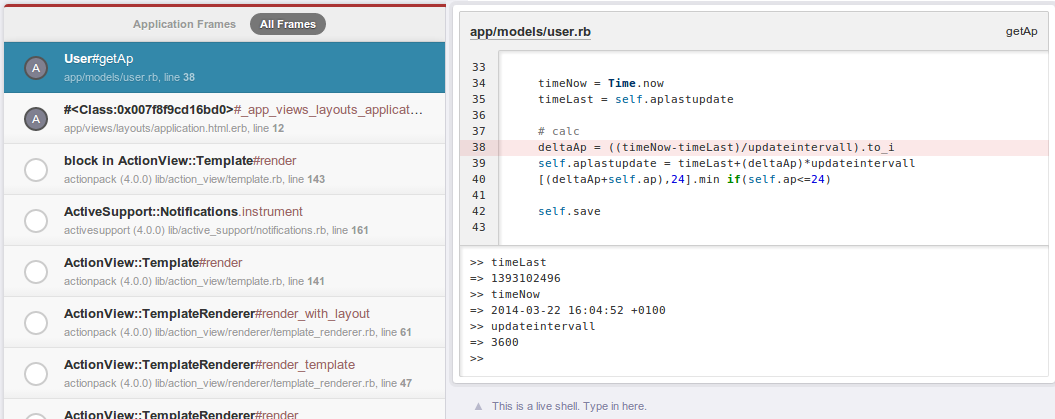
\includegraphics[width=155mm]{images/ch5_img08_livebinding.png}
\caption{Interaktives Debugging mit \glqq better\_errors\grqq{} und \glqq binding\_of\_caller\grqq{}}
\label{img:ch5_img08_livebinding}
\end{center}
\end{figure}

Für die Entwicklung von Software ist es essentiell beliebig den Code wiederherstellen zu können und einfach neue Funktionen auszuprobieren. Diese Anforderung erfüllen Software Systeme zur Versionsverwaltung. 
Die Auswahl wurde auf ein Open-Source System gelegt. Am weitesten verbreitet sind zur Zeit Subversion und Git. Letzteres bietet Möglichkeit einer nicht linearen Entwicklung.\cite{Bird.2009}
Die Wahl fiel speziell auf Subversion, da es im Gegenzug zu CVS das Versionsschema nicht auf einzelne Dateien, sondern auf das ganze Projekt bezieht.
Dies hat den Vorteil, dass das Hinzufügen einer neuen Funktion nicht in der Hauptklasse Version 50 und in der Methodenklasse Version 70 gespeichert wird, sondern in einer gemeinsamen Version.
Somit ist es für den Entwickler möglich den Zusammenhang zwischen den einzelnen Dateien direkt zu erkennen.
Die Verwendung von Git wurde in Erwägung gezogen, aber Aufgrund der Tatsache, dass das Projekt nur einen Entwickler besitzt verworfen.  Ein späterer Transfer in ein Git-Projekt ist problemlos mit \glqq git-svn clone\grqq{} ohne weiteren Anpassungen möglich. Der Transfer ist in jedem Fall zu empfehlen, gerade wenn das Framework später mit mehreren Entwicklern weiterentwickelt werden sollte.

\section{Implementierung des Geogameframeworks}
\label{ch5:s:Implementierung}

\subsection*{Realisierung}

Nachdem alle Anforderungen, Schnittstellen und Werkzeuge des Frameworks festgelegt wurden, konnte mit der Umsetzung begonnen werden.
Wie bereits in Kapitel \ref{ch5:s:Entwurf} beschrieben lässt sich das Framework in drei Module unterteilen auf die im nachfolgenden jeweils eingegangen werden soll.

\begin{itemize}

\item GameAPI (Overpass API)
\item Beispiel Spiel
\item Evaluationstool

\end{itemize}

\subsubsection*{GameAPI}

Die GameAPI stellt die API des GameFrameworks dar. Sie wird dazu verwendet um die Spielfelder aufzubauen.
Es gibt diverse Funktionen die nach außen zur Verfügung gestellt werden.
Dabei wird unterschieden zwischen den POIs (im Beispiel Spiel: Flaggen) sowie den lokalen Händlern.
Der Aufruf der Schnittstelle erfolgt mittels REST mit nachfolgenden Parametern:
\\\\
\url{SITE\_URL/overpass\_api/getLocation.json?s=49&w=10&n=50&e=11&tag=highway=bus\_stop}
\\\\
Der Aufruf kann sowohl als GET als auch als POST Request durchgeführt werden. Die Parameter s, n, w und e sind sind Pflicht und beschreiben die angefragte Bounding Box.
S steht hierbei für South (Bounding Box -- Minimum Latitude), N für North (Bounding Box -- Maximum Latitude), W für West (Bounding Box -- Minimum Longitude) und E für East (Bounding Box -- maximum Longitude).

Der letzte Parameter Tag ist optional und beschreibt den zu verwendenden OSM Tag. Wird der Tag nicht angegeben, so wird der im Framework hinterlegte Standard Tag verwendet. Ziel ist es den Standard Wert für das darauf aufbauende Beispiel Spiel zu verwenden. Der optionalen Parameter Tag soll für die Evaluation einzelner Tags genutzt werden. Nachdem der Aufruf erfolgt ist, wird das Ergebnis als GeoJSON mit den Properties zurückgeliefert.
\\ %% settings for current code
\lstset{
   language=JavaScript,
   backgroundcolor=\color{white},
   extendedchars=true,
   basicstyle=\scriptsize\ttfamily,
   showstringspaces=false,
   showspaces=false,
   frame=single,
   numbers=left,
   numberstyle=\scriptsize,
   numbersep=9pt,
   tabsize=2,
   breaklines=true,
   showtabs=false,
   captionpos=b
}

\begin{lstlisting}[caption=GeoJSON Response Location (Reduziert), label=code:ch5:geojson01]
{
  "type": "FeatureCollection",
  "features": [
    {
      "type": "Feature",
      "geometry": {
        "type": "Point",
        "coordinates": [
          10.8748794,
          49.9002723
        ]
      },
      "properties": {
        "popupContent": "Test",
        "id": "301967628",
        "user_id": "neutral",
        "prestige": 0
      }
    }
  ]
}
\end{lstlisting}

Wie in Code \ref{code:ch5:geojson01} zu sehen ist die Antwort der API analog zur GeoJSON Spezifikation.\cite{Butler.2008}
In jedem Fall enthält ein GeoJSON ein Objekt. Enthält das GeoJSON mehr als ein Objekt, so sind diese in einer FeatureCollection gesammelt. Diese wiederum enthält Objekte.
Jedes Objekt nimmt einen der nachfolgenden Typen an:
 \glqq Point\grqq{}, \glqq MultiPoint\grqq{}, \glqq LineString\grqq{}, \glqq MultiLineString\grqq{}, \glqq Polygon\grqq{}, \glqq MultiPolygon\grqq{} oder \glqq FeatureCollection\grqq{}.
Für die Implementierung des Frameworks wurde allerdings nur Point und FeatureCollection genutzt. Die Reduzierung auf Points ist der Tatsache geschuldet, dass durch die Transformation in virtuelle Nodes und die Spielelemente als solche nur als Punkt existieren. Daher ist das passendste Element im GeoJSON ebenfalls ein Point. Neben den Koordinaten des Punktes können zusätzlich weitere Attribute frei definiert werden. Diese sind für das Gameframework id, user\_id und prestige. Die id beschreibt die virtuelle Node Id des OSM Objektes. Diese enthält die Information von welchem Node das Objekt abstammt. In diesem Fall lässt sich anhand der Zahl erkennen, dass es sich hierbei um ein Node handelt, da die Bitmaske nicht verändert wurde. Das Attribut user\_id beschreibt den Besitzer des Elementes. Für das Beispiel Spiel wurde hier keine Ids sondern die Stati \glqq neutral\grqq{},\glqq owner\grqq{} und \glqq foe\grqq{} bestimmt. Mit einer einfachen Anpassung einer Zeile im Framework könnte auch direkt die Id des Spielers ausgegeben werden. Sofern die Schnittstelle ohne Session von extern aufgerufen wird, gibt es nur den Zustand \glqq neutral\grqq{} oder \glqq foe\grqq{}, da ein Anonymer Zugriff keinem eingeloggten User zugeordnet wird. Ist hingegen ein User über das Beispiel Spiel authentifiziert, so erhält er zusätzlich die Information, ob die aktuelle Flagge in seinem Besitz ist.
Das Attribut Prestige gibt den aktuellen Prestige-Wert der Flagge zurück. Im Codebeispiel handelt es sich um eine neutrale Flagge, die daher den Wert 0 hat. Eine Aussage ob ein Objekt persistiert wurde oder nicht, kann bei Verwendung der API nicht gemacht werden. Dies ist aber auch nicht notwendig, da 
die Persistierung transparent\footnote{im englischen Sinne} vor dem Spieler und der Schnittstelle ist.

Die nächste Schnittstelle stellt die Händlerschnittstelle dar. Über diese können die Händler in einer vorgegebenen Bounding Box abgefragt werden, analog zu den Flaggen.
\\\\
\url{SITE\_URL/vendors/getVendors.json?s=49&w=10&n=50&e=11}
\\\\
Im Gegensatz zu einem Spielelement enthält das GeoJSON des Händlers allerdings weniger Attribute, wie in Codebeispiel \ref{code:ch5:geojson02} zu sehen.
\\
\begin{lstlisting}[caption=GeoJSON Response Vendor (Reduziert), label=code:ch5:geojson02]
{
        "type": "Feature",
        "geometry": {
            "type": "Point",
            "coordinates": [10.869845151901245, 49.902191491264695]
        },
        "properties": {
            "popupContent": "Insel 11"
        },
        "id": 2
    }
\end{lstlisting}

Die Standardattribute sind gleich, jedoch wurden die Properties reduziert. \glqq popupContent\grqq{} beschreibt den Inhalt des Popup-Fensters. In diesem Fall werden hier die Namen der Händler ausgegeben. Darüber hinaus hat auch jeder Händler eine Id. Diese sind jedoch nicht an OSM Elemente gebunden sondern für das Framework spezifisch.

\subsubsection*{Beispiel Spiel}

Das Beispiel Spiel stellt eine Proof of Concept Implementierung dar, welche auf dem Gameframework aufbaut. Es dient vor allem zum Test des Frameworks und kann später ausgebaut oder ersetzt werden. Das Beispiel Spiel lässt sich in drei Bereiche aufteilen. Zunächst wurde das Spielfeld mittels Leaflet implementiert.

\begin{figure}[H]
\begin{center}
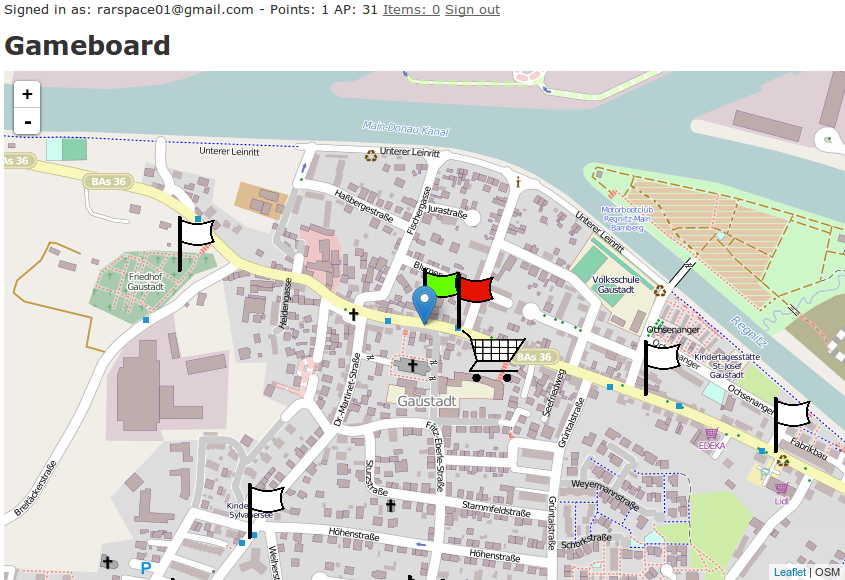
\includegraphics[width=150mm]{images/ch5_img09_gameboard.png}
\caption{Grundansicht -- Spielfeld}
\label{img:ch5_img09_gameboard}
\end{center}
\end{figure}

Das Spielfeld ist in Abbildung \ref{img:ch5_img09_gameboard} zu sehen. In der initialen Sicht wird das Spielfeld mittels HTML5 Geo Api auf die aktuelle Position zentriert. Die Karte zeigt die Standard OSM Tiles (Mapnik). Diese können beliebig ersetzt werden. Gerade in Innenstädten kann es sinnvoll sein ein anderes Rendering zu verwenden. Eine Übersicht der kostenlosen Tile-Server ist unter \url{http://wiki.OpenStreetMap.org/wiki/Tiles} zu finden. Möchte man über diese hinaus andere Styles verwenden und nicht selbst einen Tile-Renderingserver aufsetzten, so ist es zu empfehlen auf Dienste wie z.\,B. MapBox\footnote{\url{https://www.mapbox.com/}} zurückzugreifen. Auf der Karte selbst sind per Layer die Spielelemente, sowie Händler eingebunden.
Bewegt der Spieler den Kartenbereich oder bewegt er sich physisch fort, so werden die Daten nachgeladen. Die Daten werden mittels GameAPI über das Framework ausgelesen und als GeoJSON eingebunden. Möchte nun der Spieler mit den Spielelementen interagieren, so muss er nur auf das Element klicken. Im Beispiel Spiel öffnet sich dann je nach Elementtyp entweder die Übersicht der jeweiligen Flagge oder aber der Händler. Durch die Interaktion kann sich der Spieler über den aktuellen Prestige-Stand informieren, sowie die Flagge angreifen. Letzteres kann der Spieler allerdings nur, wenn er sich im Umkreis von 40 Metern zur Flagge befindet. Ein AJAX Request beim Angriff des Spielers, stellt dies sicher. Der Aktionsradius von 40 Meter stellt sicher, dass auch bei einer höheren GPS-Ungenauigkeit der Spieler trotzdem mit der Umgebung interagieren kann.
Beim Händler erhält der Spieler eine Übersicht über die verfügbaren Items. Im Gegensatz zu den Flaggen werden die Informationen der Händler nicht direkt beim Aufruf des Spielfeldes geladen. Stattdessen werden die Daten über die vorhandenen Items explizit für den jeweiligen Händler angefordert. Somit wird sichergestellt, dass die Synchronisierung möglichst zeitnah ist und der Spieler eine aktuelle Übersicht über das Inventars des virtuellen Händlers erhält.

Den aktuellen Punktestand kann der Spieler der oberen Statusleiste entnehmen. Dieser berechnet sich anhand aller Flaggen die der Spieler eingenommen hat. Dank Active Record in Verbindung mit Rails kann die Abfrage stark vereinfacht werden werden:
\\
\lstset{
   language=Ruby
}

\begin{lstlisting}[caption=Ruby - Abfrage der Spielerpunkte, label=code:ch5:activerecord01]
points = Flag.sum(:prestige, :conditions => ['user_id = ?',self.id])
\end{lstlisting}

Direkt daneben ist die Anzeige für die verbliebenen Aktionspunkte. Diese werden alle 60min um eins erhöht, bis diese 24 Aktionspunkte erreichen. Der letzte Punkt stellt die Item-Übersicht dar. Über diese kann sich der Spieler seine aktuellen Items anzeigen lassen und je nach Bedarf  verwenden. Die Items werden erst mit einem Klick auf das Inventar explizit per AJAX nachgeladen. Die Anzahl der Items kann der Spieler zu jeder Zeit in der Statusleiste sehen.
\\\\
Im Gegenzug dazu gibt es die Oberfläche für die Pflege der einzelnen Händler. Hierfür werden als Basis die durch Scaffolding generierten Formulare verwendet. Diese wurden um zusätzliche Funktionen, wie einem Leaflet Map Picker und dem dazugehörigen JavaScript Code ergänzt. Der Spielleiter sich eine Übersicht der Händler über die nachfolgende URL aufrufen:
\\\\
\url{SITE\_URL/vendors}
\\\\
In der Übersicht kann er bestehende Händler direkt löschen, neue anlegen oder bestehende bearbeiten. 
Legt der Spielleiter einen Händler an, so wird ihm nicht nur eine Liste an Attributen angezeigt, sondern er erhält auch eine Leaflet Karte, die auf der aktuellen Position zentriert ist. Über diese kann er frei auf der Karte einen Marker für die Position des Händlers setzen. Intern werden die Koordinaten des Markers gespeichert und in der Datenbank hinterlegt. Möchte der Spielleiter nun einen der Händler bearbeiten, wird das Formular wieder aufgerufen und mit den Daten aus der Datenbank gefüllt. Gleiches gilt auch für die Leaflet-Karte auf der der zuvor gespeicherte Marker hinterlegt wurde. In diesem Modus hat der Spielleiter zudem die Möglichkeit Items direkt dem Händler zuzuweisen, die dann später zum Verkauf stehen. Der Einfachheit halber werden alle noch nicht zugewiesenen Items angezeigt und können mit einem einfachen Klick hinzugefügt werden. Hierfür sind die Controller für die Händler-Klasse erstellt worden, die das Kaufen und Zuweisen von Items ermöglichen.

Über die nachfolgende URL, findet die Pflege der Items statt:
\\\\
\url{SITE\_URL/items}
\\\\
Auf dieser Seite erstellt der Spielleiter alle Items, die den Händlern zur Verfügung stehen sollen. Es handelt sich ebenfalls um ein, durch Scaffolding erzeugtem, Formularmuster zur Pflege der einzelnen Daten. Jedes Item ist dabei explizit als Objekt angelegt und kann einem Item-Typ angehören. Das Anpassen der Items ist nach der Erstellung möglich. Im Zuge des Beispiel Spiels wurde auf eine umfangreiche Rollen und Rechtevergabe verzichtet, da der Fokus auf den Spielelemente lag. Diese können später bei Bedarf ergänzt werden, sofern ein Einsatz dieser notwendig ist.

\subsubsection*{Evaluationstool}

Das Evalutationstool verwendet die zuvor in der GameAPI beschriebene Schnittstelle um Spielfelder zu bewerten bzw. zu evaluieren. Hierfür wird die zusätzliche Möglichkeit genutzt konkrete Tags zu einer Bounding Box abzufragen. Für eine Evaluation verwendet das Tool eine vorgegebene Liste an Key-Value Paaren und eine Geo-Koordinate, die zu einer Bounding Box erweitert wird. Basierend auf den in Kapitel \ref{ch:CH6_qualtiy_of_gameboards} beschriebenen Ansätzen werden die Spielfelder jeweils evaluiert. Für die Evaluation der Spielfelder müssen die Entfernung zwischen den einzelnen Punkten berechnet werden. Hierbei werden nicht die euklidische Distanz zwischen den Geo-Koordinaten berechnet, sondern es muss die reale Distanz auf dem Straßennetz berechnet werden. Da der Spieler sich nicht nur per Auto, sondern auch per Fahrrad und im besten Fall zu Fuß fortbewegt, ist ein Fußgängerrouting notwendig. Nur für Fußgänger zugängliche Wege, müssen ebenfalls beachtet werden. Da OpenStreetMap im Vergleich zu Google Maps im Hinblick auf den Datenumfang an dieser Stelle einen Vorteil hat, wird auf OSM zurückzugreifen. Durch den Umfang und Anzahl der Abfragen ist es sinnvoll diese nicht an einen Onlinedienst zu stellen, sondern diese offline mit einem dedizierten Routing durchzuführen. Für das Offline-Routing mit OSM gibt es diverse Bibliotheken. Aufgrund der Anforderung möglichst viele Abfragen zeitnah durchzuführen, wurde sich für das Tool GraphHopper entschieden. Dieses bietet ein vollständiges Offline Routing auf Basis von OSM Rohdaten.\cite{Karich.2014} Hierfür erstellt GraphHopper zunächst die Indexdateien, auf denen dann später das Routing stattfindet. Diese enthalten in binärer Form die aggregierten Pfadkosten des Netzwerkes.

Mit Hilfe von GraphHopper ist es nun möglich schnelle Abfragen durchzuführen. Da die GraphHopper Bibliothek selbst nicht für Parallelisierung ausgelegt ist, wurde das Evaluationstool optimiert um die Ressourcen eines Rechners/Servers vollständig auszunutzen. Dadurch kann die Laufzeit bei mehreren Tags je nach Anzahl der vorhandenen CPUs auf $\frac{1}{lc}$ verkürzt werden. Hierbei steht lc für die Anzahl der logischen CPUs. Bei einer Laufzeit von $\mathcal O(n^2)$ ist dies unerlässlich.
Da GraphHopper in Java realisiert wurde, wurde das Evaluationstool analog dazu ebenfalls in Java entwickelt.

\subsection*{Tests}

Da das Framework später für verschiedene Spiele genutzt werden soll, muss dieses getestet werden.
Hierbei wird unterschieden zwischen Low-Level-Tests und High-Level-Tests.\cite{Pol.2002}
Unter Low-Level-Tests sind solche Test zu verstehen, die während der Implementierung an Teilen des Systems stattfinden. Bei High-Level-Tests wird das komplette System getestet. Einer der Low-Level-Tests ist der Modultest. Bei diesem werden einzelne Module im Programm getestet.  

Für das Gameframework wurden die einzelnen Module unabhängig voneinander getestet. Zunächst wurden speziell die Schnittstellen zu OSM und Overpass getestet. Hierbei wurden vor allem  die Übergabeparameter, sowie das Datenformat kontrolliert. Die korrekte Interpretation der Daten war ein weiterer Punkt, der überprüft wurde.
Nachdem die die GameAPI mit ihrer Transformation der OSM Elemenete in Spielelemente implementiert wurde, ist das Beispiel Spiel darauf aufgebaut worden. Hierzu wurde die korrekte Transformation der Elemente anhand von speziellen Tags manuell überprüft. Für die Tags wurde auf \url{http://taginfo.openstreetmap.org} zurückgegriffen. Die Seite bietet einen statistischen Überblick aller Tags in OSM sowie die Verteilung auf die Elemente Relation, Way und Nodes. Der Test erfolge anhand von Key-Value Paaren, die jeweils explizit nur als einer der drei Typen bevorzugt gemappt werden.

Das Beispiel Spiel selbst musste ebenfalls getestet werden. Da ein ortsbezogenes Spiel als Grundlage die Position des Spielers verwendet, ist ein Debugging unterwegs schwierig. Aufgrund dessen ist es am besten die GPS-Koordinate zu simulieren. Hierfür gibt es Plugins für die am weitesten verbreiteten Browser, wie Chrome oder Firefox. Mit deren Hilfe kann die Position, welche die HTML5 Geo-API zurück liefert, verändert werden. Darüber hinaus ist es auch möglich die Genauigkeit der GPS Position, sowie das Bewegungs-Event zu triggern. Mit Hilfe von diesen können alle ortbezogenen Funktionen des Beispiel Spiels auch direkt während der Entwicklung getestet werden.
Für die Nutzung des Spieles auf Smartphones eignet sich darüberhinaus der Einsatz von Emulatoren. Für Android und FirefoxOS sind diese frei verfügbar. Für iOS fallen jährliche Gebühren an und der Emulator inkl. SDK ist nur unter der neusten Mac OS X Version verfügbar.

Tests für das Evaluationstool wurden vorwiegend für die Laufzeit sowie der Bewertung von Spielfeldern durchgeführt.
Konkrete Unit-Tests wurden für das Framework aus Zeitgründen nicht entwickelt, sollten aber als nächster wichtiger Punkt implementiert werden.

Als High-Level bzw. Blackbox Test wurden die in den Usecase Diagramm beschriebenen Anwendungsfälle getestet. Es wurden daher die Funktionen, die den jeweiligen Akteuren zur Verfügung stehen, ohne aktives Debugging des Quellcodes geprüft.

\subsection*{Probleme}

Während der Umsetzung wurde auf einige Besonderheiten gestoßen, welche eine spezielle Anpassung oder Überlegung erfordert haben. Im Nachfolgenden soll kurz auf diese eingegangen werden, um die Erkenntnisse festzuhalten. Idealerweise können diese in zukünftigen Untersuchungen und Implementierungen vermieden bzw. umgangen werden.

Ein erster Aspekt ist die Spezifikation der GeoJSON. Standardmäßig werden Koordinaten in der Reihenfolge Latitude, Longitude angegeben.\cite{Schoeneberger.2002,Barzegar.1996,Maling.1991,}
Die GeoJSON Spezifikation hingegen sieht im Kontrast zum de facto Standard vor, dass zuerst die Longitude und dann die Latitude genannt wird.\cite{Butler.2008} Ist dies nicht bekannt, kann dies zu einigem Aufwand führen, der vermieden werden kann.

Eine weitere Problematik stellten die Bitmasken im Zuge des Transformationsprozesses der Relations und Ways zu virtuellen Nodes dar. Die Verwendung einer 64Bit Maske führte im Zuge der Verwendung von Javascript zu Problemen. Dies äußerte sich darin, dass die Ids nach der Interpreation auf unerklärlicher Weise veränderte Werte annahmen. So kamen Abweichungen im Wert von bis zu 100 Einheiten zu Stande. Nach längeren Debug Aufwänden wurde herausgefunden, dass die implizite Typisierung in JavaScript den Ganzzahlenwert der Id intern als Gleitkommazahl transferiert und dadurch unbewusster Weise die 51Bit überschreitet nach denen die Mantisse der Gleitkommazahl beginnt. Durch diese Verschiebung wurden die hinteren Bits beim Auslesen des long Wertes vernachlässigt. Um dieses Problem zu umgehen gibt es zwei Möglichkeiten. Entweder man teilt die Zahl auf Basis des 64Bit long Wertes in zwei 32Bit Integer Werte und legt diese in zwei Zahlen in JS ab. Da in diesem Fall in JavaScript keine arithmetischen Operationen auf der Id durchgeführt werden sollen empfiehlt es sich die Id explizit als String auszugeben. Dadurch interpretiert JavaScript diese nicht als Zahl und versucht diese nicht umzuwandeln.

Ein weiterer Punkt stellt Turbolinks dar. Turbolinks ist ein Gem, welches Standardmäßig in Rails aktiv ist. Es sorgt dafür, dass bei einer Interaktion mit der Seite nicht die komplette Seite neu geladen wird, sondern nur die Teile des Html Codes, welche sich geändert haben.\cite{Gamble.2013}
Die Problematik die damit einhergeht sind Ajax Requests, welche über normale href links angestoßen werden. Eine typische Verwendung ist z.\,B.:
\\
\lstset{
   language=Html
}

\begin{lstlisting}[caption=a href HTML Code, label=code:ch5:html01]
<a href="#" onClick="saveItem(1);">Save</a>
\end{lstlisting}

Allerdings führt der Klick auf \glqq Save\grqq{} in diesem Fall zu einem Neuladen der Seite durch Turbolinks. Befindet sich an dieser Stelle aber ein Javascriptcode mit einem Ajax Request, dann wird die Seite neu geladen anstatt dass der Code ausgeführt wird. Dies ist speziell bei Skripten unvorteilhaft, die z.\,B. eine Aktualisierung von Werten auf der Seite vornehmen.
Um dies zu vermeiden muss Turbolinks explizit angewiesen werden, bei \glqq a href\grqq{}-Links nicht aktiv zu werden. Dies kann pro Link individuell gesetzt werden:
\\
\begin{lstlisting}[caption=a href HTML Code - Turbolinks deaktiviert, label=code:ch5:html02]
<a href="#" data-no-turbolink onClick="saveItem(1);">Save</a>
\end{lstlisting}

Dadurch wird sichergestellt, dass der JavaScript Code ausgeführt wird und nicht einfach die Seite neu geladen wird.

Ein letzter Punkt, der zu Problemen führen kann ist der \glqq Zurück\grqq{}-Button im Browser.
Durch diesen wird die vorherige Seite wieder aufgerufen, allerdings deren Javascriptcode nicht noch einmal ausgeführt, wie beim Laden der Seite. Als Resultat werden diverse Event-Listener nicht aufgerufen. Speziell \glqq OnDocumentReady\grqq{} wird nicht aufgerufen. Sofern dies nicht in der Entwicklung berücksichtigt wird, kann dies dazu führen, dass die Seite vom Benutzer in einem nicht definierten geführt wird.
